De belangrijkste applicatie om settings in Windows te wijzigen is Settings. Het is de opvolger van Control Panel. Vanuit Settings kan je ook bij help en troubleshooting komen, dat het de centrale plek is om Windows te beheren.

Er zijn verschillende manieren om Settings te openen:
\begin{itemize}
\item Gebruik de Windows-toets + i
\item Klik op start (windows-icon) en selecteer Settings
\end{itemize}

\begin{minipage}[t]{\linewidth}
\raggedright
\adjustbox{valign=t}{%
	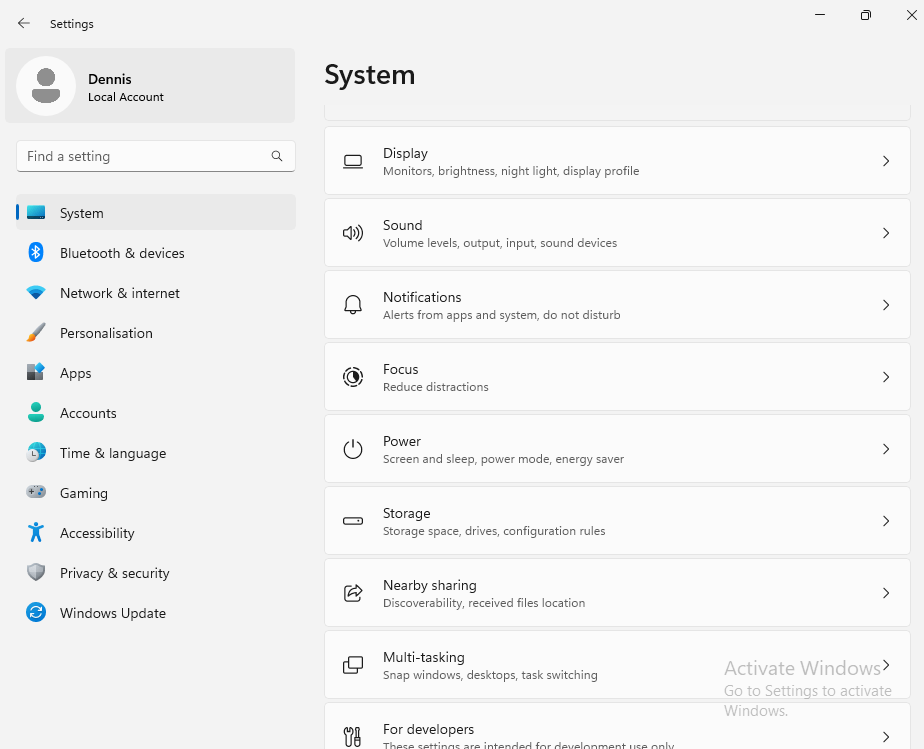
\includegraphics[width=0.99\linewidth]{settings.png}%
}
\end{minipage}

